\documentclass[12pt, a4paper]{article}
\usepackage[utf8]{inputenc}
\usepackage[T1]{fontenc}
\usepackage[brazil]{babel}
\usepackage{geometry}
\usepackage{amsmath}
\usepackage{amssymb}
\usepackage{graphicx}
\graphicspath{{graficos/}}
\usepackage{float}
\usepackage{xcolor}
\usepackage{booktabs}
\usepackage{siunitx}
\usepackage{ragged2e}
\usepackage{listings}
\usepackage[colorlinks=true, linkcolor=black, urlcolor=black, citecolor=blue]{hyperref}

\geometry{a4paper, left=3cm, right=2.5cm, top=3cm, bottom=2.5cm}
\setlength{\parindent}{1.25cm}


\begin{document}
    \begin{titlepage}
        \centering
        
        
        
        \textbf{\large UNIVERSIDADE FEDERAL DA BAHIA} \\
        \vspace*{1.5cm}
        
\includegraphics[width=1.0\textwidth, height=0.4\textheight, keepaspectratio]{brasao_ufba.jpg}



        \textbf{\large ESCOLA POLITÉCNICA} \\
        \textbf{\large DEPARTAMENTO DE ENGENHARIA QUÍMICA} \\
        
        \vfill
        
        {\Huge\bfseries Otimização de Sistema de Bombeamento de Biodiesel} \\
        
        \vspace{1.5cm}
        
        {\Large Relatório Técnico de Análise de Custos} \\
        
        \vfill
        
        \begin{flushleft}
            \textbf{\large Elaborado por:} \\
            \vspace{0.2cm}
            Fernanda Oliveira Santos Roza \\
            Guilherme Rocha Ribeiro
        \end{flushleft}
        
        \vfill
        
        \textbf{\large Salvador, BA} \\
        \textbf{\large \today}

    \end{titlepage}

    \tableofcontents
    \newpage


    \section{Introdução}
    \justifying
    Este relatório apresenta uma análise técnico-econômica para a otimização de um sistema de transporte de biodiesel. O objetivo principal é determinar o diâmetro de tubulação que minimiza o custo total anualizado, considerando um balanço entre os custos de capital 
    (investimento na tubulação) e os custos operacionais (consumo de energia da bomba). A metodologia empregada baseia-se em princípios fundamentais da mecânica dos fluidos e em uma análise de custos simplificada, implementada em Python para identificar o ponto dentro do intervalo que minimiza o custo da operação.

    \section{Metodologia e Modelagem}

        \subsection{Descrição do Problema e Escolhas de Modelagem}
        O sistema em análise consiste no bombeamento de biodiesel através de uma tubulação de aço horizontal de $50~\mathrm{m}$ de comprimento. Além disso, O fluido precisa vencer uma altura estática de $10~\mathrm{m}$, representando a diferença de elevação a ser superada no ponto de descarga. O problema apresetado consiste em encontrar o valor do diâmetro dentro do intervalo de 0.03 m e 0.3 m que minimiza o custo total da operação.

        \subsubsection{Escolhas Metodológicas}
        \begin{itemize}
            \item \textbf{Análise Discreta de Diâmetros:} Em vez de uma otimização contínua, optou-se por avaliar um intervalo de diâmetros comerciais plausíveis (de $0.03~\mathrm{m}$ a $0.3~\mathrm{m}$) em 100 pontos distintos.
            \item \textbf{Equação de Swamee-Jain:} Para o cálculo do fator de atrito, foi escolhida a equação explícita de Swamee-Jain. Esta fórmula oferece uma aproximação da equação implícita de Colebrook-White para escoamento turbulento e evita a necessidade de solucionadores iterativos, simplificando o código. Embora seja mais precisa para $Re > 4000$, sua aplicação em toda a faixa de diâmetros foi considerada uma simplificação razoável. \cite{Swamee}
            \item \textbf{Modelo de Custo:} O custo da tubulação foi modelado como uma função quadrática do diâmetro ($C \propto D^2$), representando uma aproximação onde o custo é proporcional ao volume de material. O custo de energia foi calculado com base na operação contínua da bomba ao longo de um ano (8760 horas).
        \end{itemize}
        \vfill

        \subsubsection{Parâmetros do Sistema}
            \begin{figure}[H]
                \centering
                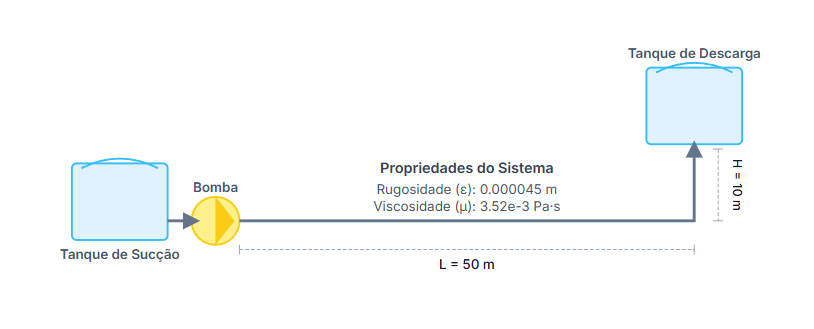
\includegraphics[width=1.0\textwidth, height=0.4\textheight, keepaspectratio]{diagrama_processo.png}
                \caption{Diagrama esquemático do sistema de bombeamento de biodiesel.}
                \label{fig:diagrama}
            \end{figure}
            Os parâmetros físicos e econômicos utilizados como base para os cálculos estão detalhados na Tabela \ref{tab:parametros}.

            \begin{table}[H]
                \centering
                \caption{Parâmetros Físicos e Econômicos do Sistema}
                \label{tab:parametros}
                \begin{tabular}{l c l}
                    \toprule
                    \textbf{Parâmetro} & \textbf{Símbolo} & \textbf{Valor} \\
                    \midrule
                    Densidade do Biodiesel SoyAB & $\rho$ & $880 ~\mathrm{kg/m^3}$ \\
                    Viscosidade Dinâmica & $\mu$ & $3.52 \times 10^{-3}~\mathrm{Pa \cdot s}$ \\
                    Vazão Volumétrica & $Q$ & $0.00333~\mathrm{m^3/s}$ \\
                    Comprimento da Tubulação & $L$ & $50~\mathrm{m}$ \\
                    Rugosidade Absoluta & $\epsilon$ & $4.5 \times 10^{-5}~\mathrm{m}$ \\
                    Altura Estática & $H_{\text{estatica}}$ & $10~\mathrm{m}$ \\
                    Eficiência da Bomba & $\eta$ & $70~\%$ \\
                    Custo da Energia & - &  $0.70~\mathrm{R\$/kWh}$ \\
                    Valor / metro & - & $300~\mathrm{R\$/ m^2}$ \\
                    \bottomrule
                \end{tabular}
            \end{table}

    \subsubsection{Cálculos e Equacionamento Completo}
    \justifying
    Para cada diâmetro $D$ no intervalo analisado, os seguintes cálculos foram realizados sequencialmente. O detalhamento das formulas pode ser encontrado em \cite{formulas}: 

        \begin{enumerate}
            \item \textbf{Velocidade do Escoamento ($v$):} Calculada a partir da vazão e da área da seção transversal ($A = \pi D^2 / 4$).
            \[ v = \frac{Q}{A} = \frac{4Q}{\pi D^2} \]

            \item \textbf{Número de Reynolds ($Re$):} Para determinar o regime de escoamento.
            \[ Re = \frac{\rho v D}{\mu} \]

            \item \textbf{Fator de Atrito ($f$):} Utilizando a equação de Swamee-Jain.
            \[ f = \frac{0.25}{\left[ \log_{10}\left( \frac{\epsilon}{3.7D} + \frac{5.74}{Re^{0.9}} \right) \right]^2} \] \

            \item \textbf{Perda de Carga por Atrito ($h_f$):} Calculada pela equação de Darcy-Weisbach.
            \[ h_f = f \frac{L}{D} \frac{v^2}{2g} \]

            \item \textbf{Altura Manométrica Total ($H$):} A altura total que a bomba precisa fornecer.
            \[ H = H_{\text{estatica}} + h_f \]

            \item \textbf{Potência da Bomba ($P$):} A potência real consumida pela bomba.
            \[ P = \frac{\rho g Q H}{\eta} \]

            \item \textbf{Custo Anual Total ($C_{\text{total}}$):} Soma dos custos de capital e operacionais.
            \[ C_{\text{total}}(D) = \underbrace{(300 \cdot D^2 \cdot L)}_{\text{Custo Tubulação}} + \underbrace{\left( \frac{P(D)}{1000} \cdot 8760 \cdot 0.70 \right)}_{\text{Custo Energia Anual}} \]
        \end{enumerate}


    \section{Resultados e Discussão}
        \subsection{Resultados da Otimização}
            O diâmetro que minimiza o custo total anual foi encontrado em \textbf{$0.0922~\mathrm{m}$} para o tubo de aço comercial, que apresenta o valor de $\epsilon$ = $4.5 \times 10^{-5}~\mathrm{m}$. Os resultados detalhados para este ponto estão descritos na Tabela
            \begin{table}[H]
                \centering
                \caption{Resultados}
                \label{tab:resultados caso1}
                \begin{tabular}{l l}
                    \toprule
                    \textbf{Parâmetro} & \textbf{Valor} \\
                    \midrule
                    Diâmetro ótimo & $0.0922~\mathrm{m}$ \\
                    Perda de carga ($h_f$) & $0.2110~\mathrm{m}$ \\
                    Potência da bomba ($P$) & $419.34~\mathrm{W}$ \\
                    Custo da tubulação & R\$ 127.57 \\
                    Custo energético anual & R\$ 2571.39 \\
                    \midrule
                    \textbf{Custo Total Anual Mínimo} & \textbf{R\$ 2698.96} \\
                    \bottomrule
                \end{tabular}
            \end{table}



        \subsection{Análise dos Gráficos}
            \begin{figure}[H]
                    \centering
                    \caption{Curva de custo total anual em função do diâmetro da tubulação.}
                    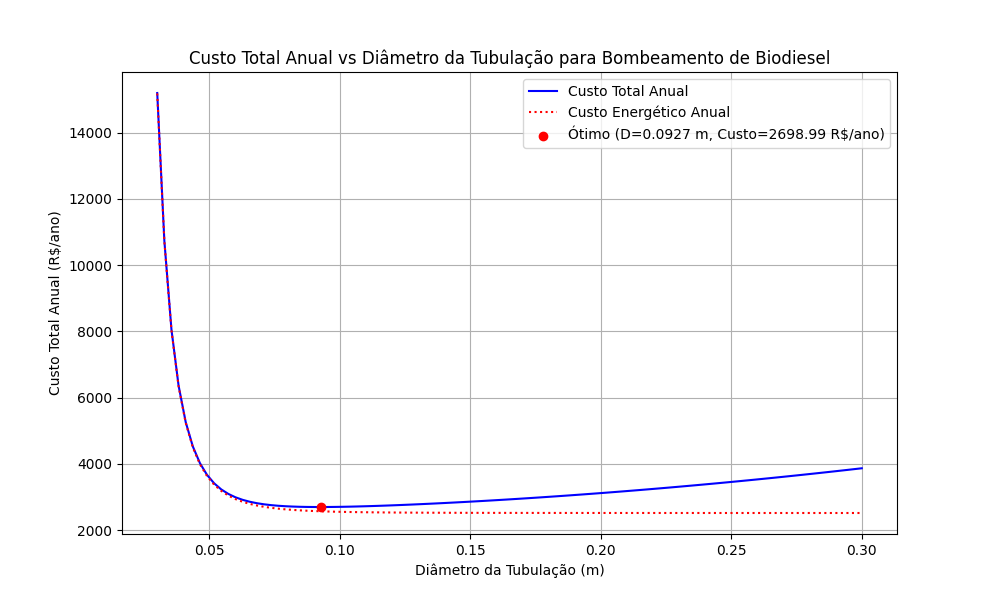
\includegraphics[width=1.0\textwidth, height=0.4\textheight, keepaspectratio]{custo_por_diametro.png}
                    \label{fig:custos_grafico}
            \end{figure}

            \begin{figure}[H]
                    \centering
                    \caption{Calculo da potência necessária em função do diametro da tubulação.}
                    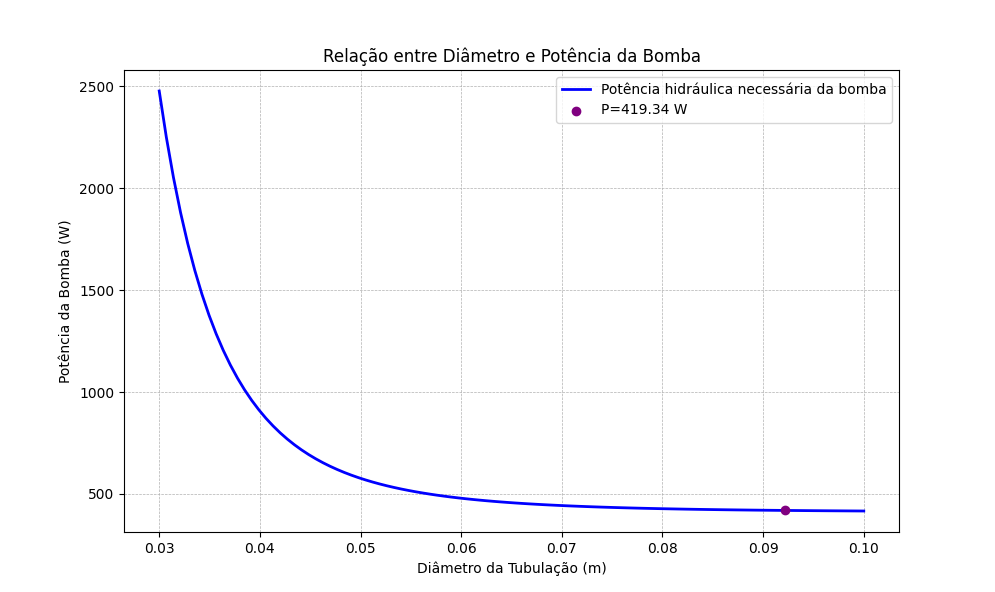
\includegraphics[width=1.0\textwidth, height=0.4\textheight, keepaspectratio]{potencia_necessaria.png}
                    \label{fig:potencia}
            \end{figure}

            \begin{figure}[H]
                    \centering
                    \caption{Calculo da resistencia do escoamento em função do diametro da tubulação.}
                    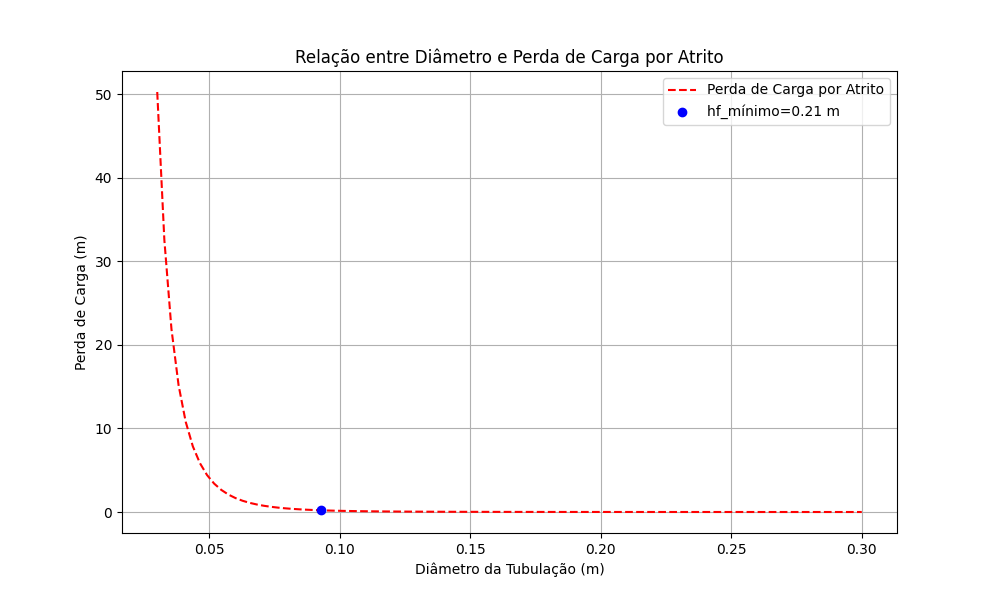
\includegraphics[width=1.0\textwidth, height=0.4\textheight, keepaspectratio]{perda_carga.png}
                    \label{fig:hf}
            \end{figure}

            A análise gráfica, permite a identificação dos seguintes pontos
            \begin{itemize}
                \item \textbf{Diâmetros próximos de 0.03 m:} Nesta faixa, o custo total é máximo. Visto que, diâmetros menores implicam em velocidades de escoamento muito mais altas. Como a perda de carga por atrito é proporcional ao quadrado da velocidade ($h_f \propto v^2$), ela aumenta drasticamente, exigindo uma potência de bombeamento oque torna o custo inviável para operações com diâmetros próximos e essa faixa do intervalo.
                \item \textbf{Diâmetro ideal de 0.0922 m} Ponto encontrado onde é minimizada o custo, potência necessaria e o valor do atrito do fluido com a tubulação
                \item \textbf{Diâmetros na faixa superior (>0.0922 m):}  Acima do ótimo, o custo da tubulação cresce quadraticamente ($300 \cdot D^2 \cdot L$)
            \end{itemize}

    \section{Conclusão}
        O estudo demonstrou com sucesso a existência de um diâmetro ótimo que minimiza o custo total anualizado de um sistema de bombeamento. A análise das curvas de custo revela que o ponto ótimo, encontrado em \textbf{0.0922 m} minimiza o custo total da operação.

        No ponto ótimo, o custo energético anual (R\$ 2.571.39) representa aproximadamente 95.2\% do custo total anual (R\$ 2.698.96), enquanto o custo da tubulação (R\$ 127,57) corresponde aos 4.8\% restantes. Isso evidencia que, para este sistema, o gasto operacional com energia é o fator mais impactante no custo total a longo prazo. Portanto, a abordagem quantitativa de otimização é essencial para garantir não apenas a viabilidade econômica, mas também a eficiência energética do projeto.


        \subsection*{Sugestões para Trabalhos Futuros}
            \begin{itemize}
                \item \textbf{Análise de Custo de Vida Útil (LCCA):} Incluir custos de manutenção, depreciação e o valor do dinheiro no tempo.
                \item \textbf{Perdas de Carga Localizadas:} Adicionar ao cálculo as perdas de carga devido a acessórios como válvulas e curvas.
                \item \textbf{Curva da Bomba:} Integrar a curva característica da bomba (Altura vs. Vazão) para garantir que o ponto de operação seja viável.
                \item \textbf{Análise de Sensibilidade:} Avaliar como o diâmetro ótimo varia com mudanças nos parâmetros de entrada.
            \end{itemize}
    
    \begin{thebibliography}{9}
        \bibitem{diesel_density}
            Maria Jorge Pratas, Samuel V. D. Freitas, et al; 
            \text{Biodiesel Density: Experimental Measurements and Prediction Models}, Energy Fuels, 2011.

        \bibitem{formulas}
            Jukka Kiij¨arvi, \text{Darcy Friction Factor Formulae in TurbulentPipe Flow}, 2011, Cap 2.

        \bibitem{Swamee}
            Swamee, P., Jain, A.,
            \text{Explicit equations for pipe-flow problems}, Journal of the Hydraulics Division (ASCE), 102 (5), 1976, pp. 657–664.

        \bibitem{Haaland}
            Haaland, S., 
            \text{Simple and Explicit Formulas for the Friction Factor in Turbulent flow.} Transactions of ASME, Journal of Fluids Engineering,103, 1983, pp. 89–90.

    \end{thebibliography}
\end{document}